\textbf{Целью второй лабораторной работы} является освоение возможностей программы Microsoft Project для работы с ресурсами.

\section*{Задание для тренировки}

Для добавления информации о ресурсах во временный план проекта, подготовленного в лабораторной работе № 1, в лист ресурсов был добавлен трудовой ресурс <<Исполнитель>> со стандартной ставкой 120 рублей в день. Так как к реализации проекта привлекалось не более 11 исполнителей, значение максимума единиц установлено в 1100\%. Заполнение ресурсного листа показано на рисунке \ref{img:task0-executor}.

\begin{figure}[H]
	\begin{center}
		
\includegraphics[scale=0.45]{inc/img/task0-executor.jpg}
	\end{center}
	\captionsetup{justification=centering}
	\caption{Заполнение ресурсного листа}
	\label{img:task0-executor}
\end{figure}

Назначение ресурсов на задачи было произведено в соответствии с таблицей \ref{tab:tasks}. Пример назначения ресурса --- назначение двух исполнителей работе A, представлен на рисунке \ref{img:task0-assignment}. 

\begin{table}[h]
    \caption{Назначение ресурсов на задачи}\vspace{-0.5cm}\fontsize{12pt}{12pt}\selectfont
    \begin{center}
        \begin{tabular}{|c|c|}
        		\hline
            \textbf{Название работы} & 
            \textbf{Количество исполнителей (чел.)} \\ \hline
            Работа A & 2 \\ \hline
            Работа B & 6 \\ \hline
            Работа C & 2 \\ \hline
            Работа D & 5 \\ \hline
            Работа E & 4 \\ \hline
            Работа F & 6 \\ \hline
            Работа G & 1 \\ \hline
            Работа H & 7 \\ \hline
            Работа I & 1 \\ \hline
            Работа J & 4 \\ \hline
        \end{tabular}
    \end{center}
    \label{tab:tasks}
\end{table}

\begin{figure}[H]
	\begin{center}
		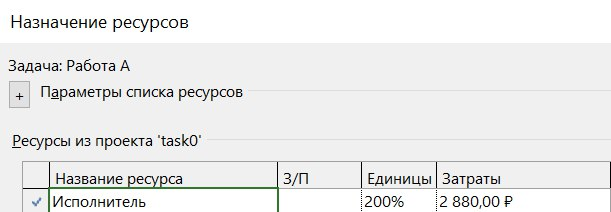
\includegraphics[scale=0.5]{inc/img/task0-assignment.jpg}
	\end{center}
	\captionsetup{justification=centering}
	\caption{Пример назначения ресурса задаче}
	\label{img:task0-assignment}
\end{figure}

Диаграмма Ганта, полученная после назначения задачам исполнителей, приведена на рисунке \ref{img:task0-diagram1}.

\begin{figure}[H]
	\begin{center}
		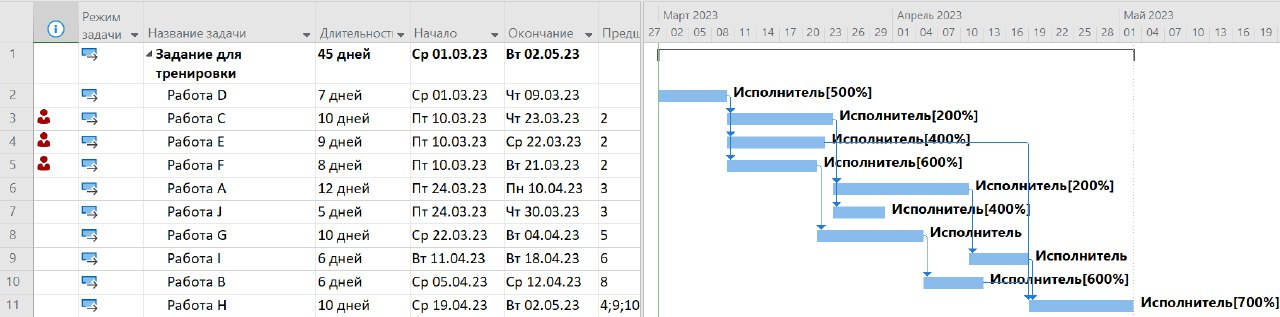
\includegraphics[scale=0.48]{inc/img/task0-diagram1.jpg}
	\end{center}
	\captionsetup{justification=centering}
	\caption{Диаграмма Ганта, полученная после назначения задачам исполнителей}
	\label{img:task0-diagram1}
\end{figure}

Так как на третий день реализации работы В арендовалось оборудование по ставке 5 000 рублей в неделю, на установку и наладку которого было выделено 2 000 рублей, в лист ресурсов был добавлен трудовой ресурс <<Оборудование>>, как показано на рисунке \ref{img:task0-equipment}.

\begin{figure}[H]
	\begin{center}
		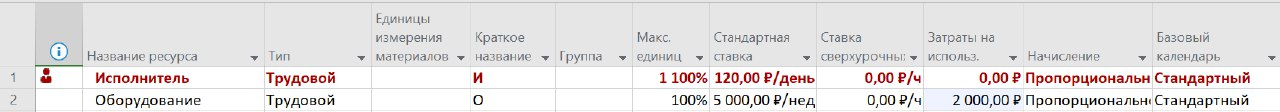
\includegraphics[scale=0.45]{inc/img/task0-equipment.jpg}
	\end{center}
	\captionsetup{justification=centering}
	\caption{Лист ресурсов после добавления оборудования}
	\label{img:task0-equipment}
\end{figure}

Поскольку оборудование арендовалось с третьего по шестой день реализации работы B для ресурса была установлена задержка в два дня, что представлено на рисунке \ref{img:task0-delay}.

\begin{figure}[H]
	\begin{center}
		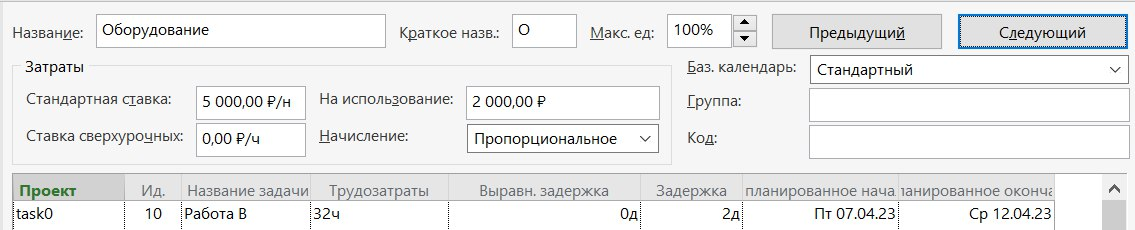
\includegraphics[scale=0.45]{inc/img/task0-delay.jpg}
	\end{center}
	\captionsetup{justification=centering}
	\caption{Установка задержки ресурсу}
	\label{img:task0-delay}
\end{figure}

Диаграмма Ганта, полученная после назначения задаче оборудования, приведена на рисунке \ref{img:task0-diagram2}.

\begin{figure}[H]
	\begin{center}
		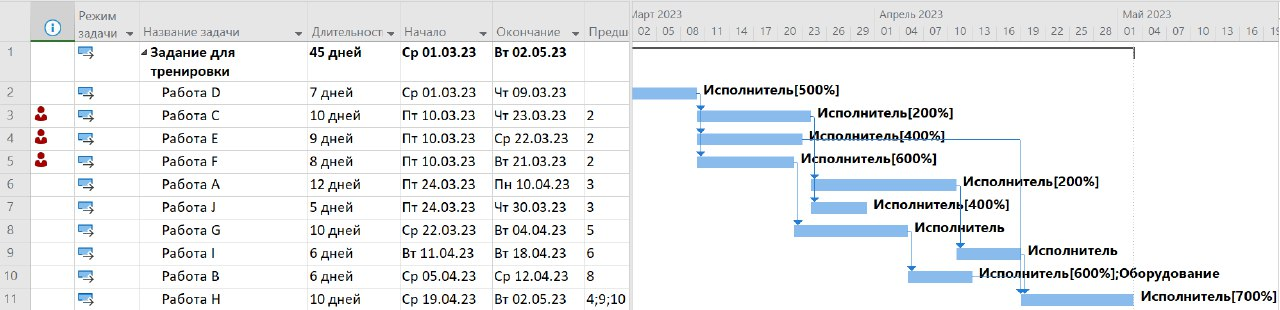
\includegraphics[scale=0.48]{inc/img/task0-diagram2.jpg}
	\end{center}
	\captionsetup{justification=centering}
	\caption{Диаграмма Ганта, полученная после назначения задаче оборудования}
	\label{img:task0-diagram2}
\end{figure}

Для ресурса <<Исполнитель>> возникли перегрузки. Наличие перегрузок связано с тем, что данный ресурс задействован при выполнении работ С, E, F, сроки реализаций которых накладываются, как показано на рисунке~\ref{img:task0-overload}.

\begin{figure}[H]
	\begin{center}
		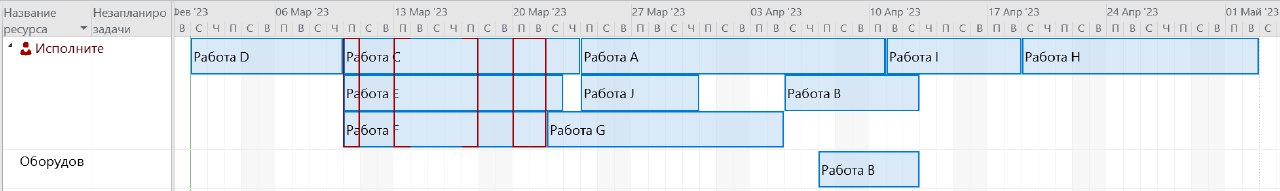
\includegraphics[scale=0.45]{inc/img/task0-overload.jpg}
	\end{center}
	\captionsetup{justification=centering}
	\caption{Возникновение перегрузок}
	\label{img:task0-overload}
\end{figure}

На рисунке \ref{img:task0-budget} представлены затраты на проект.

\begin{figure}[H]
	\begin{center}
		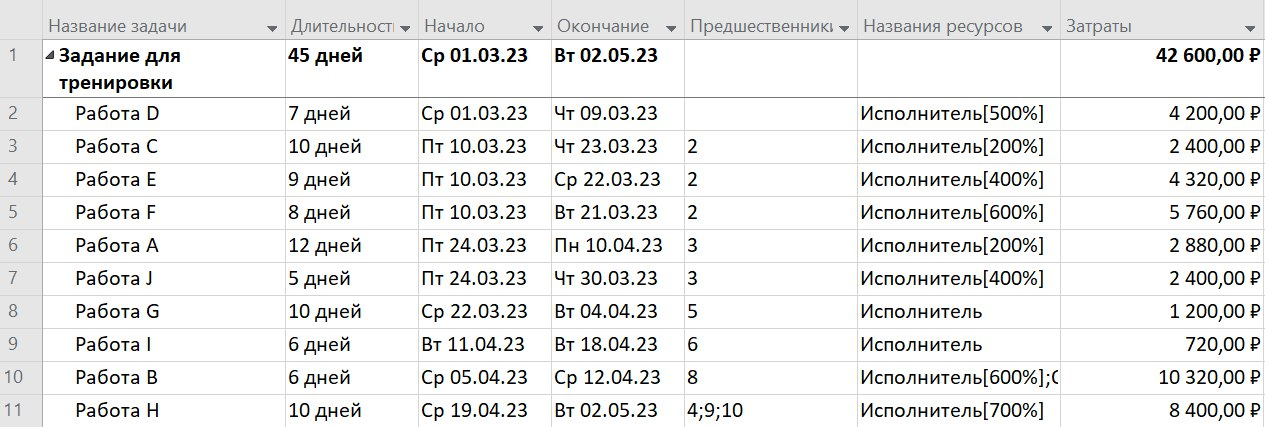
\includegraphics[scale=0.45]{inc/img/task0-budget.jpg}
	\end{center}
	\captionsetup{justification=centering}
	\caption{Затраты на проект}
	\label{img:task0-budget}
\end{figure}

Из полученного результата видно, что бюджет проекта составил 42 600~рублей.

\section*{Содержание проекта}

Команда разработчиков из 16 человек занимается созданием карты города на основе собственного модуля отображения. Проект должен быть завершен в течение шести месяцев. Бюджет проекта: 50 000 рублей.

\section*{Задание 1}

В ресурсный лист были добавлены ресурсы, приведенные на рисунке \ref{img:task1-list}.

\begin{figure}[H]
	\begin{center}
		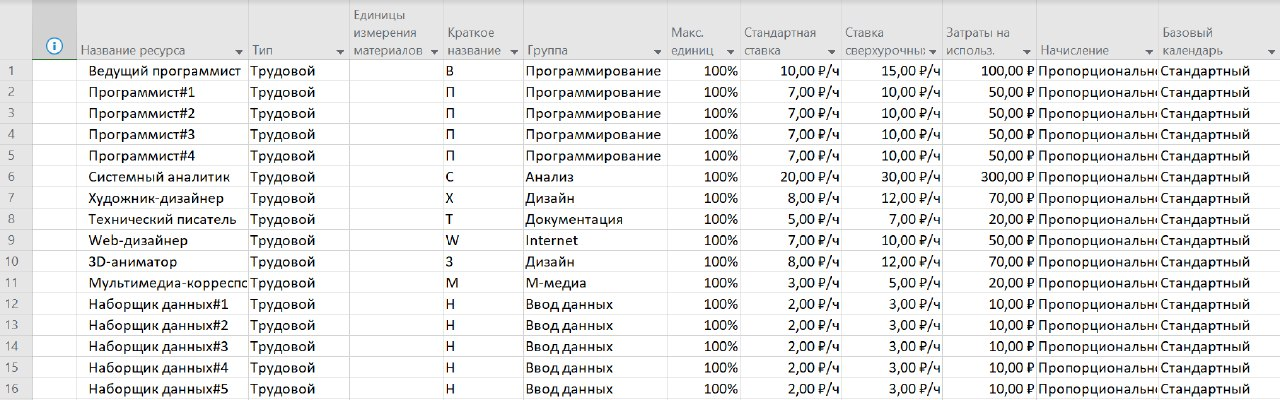
\includegraphics[scale=0.45]{inc/img/task1-list.jpg}
	\end{center}
	\captionsetup{justification=centering}
	\caption{Заполненный лист ресурсов}
	\label{img:task1-list}
\end{figure}

\section*{Задание 2}

Полученная после назначения ресурсов задачам диаграмма Ганта показана на рисунке \ref{img:task2-diagram}.

\begin{figure}[H]
	\begin{center}
		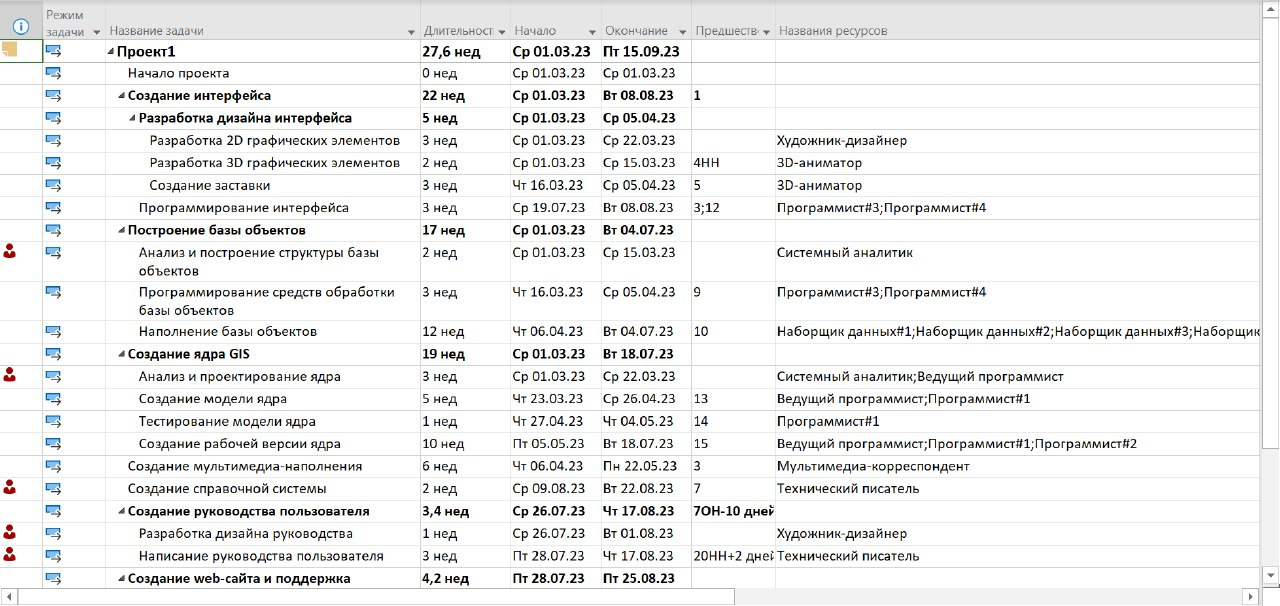
\includegraphics[scale=0.45]{inc/img/task2-diagram.jpg}
	\end{center}
	\captionsetup{justification=centering}
	\caption{Диаграмма Ганта, полученная после назначения ресурсов задачам}
	\label{img:task2-diagram}
\end{figure}

На рисунке \ref{img:task2-overload} представлены возникшие перегрузки.

\begin{figure}[H]
	\begin{center}
		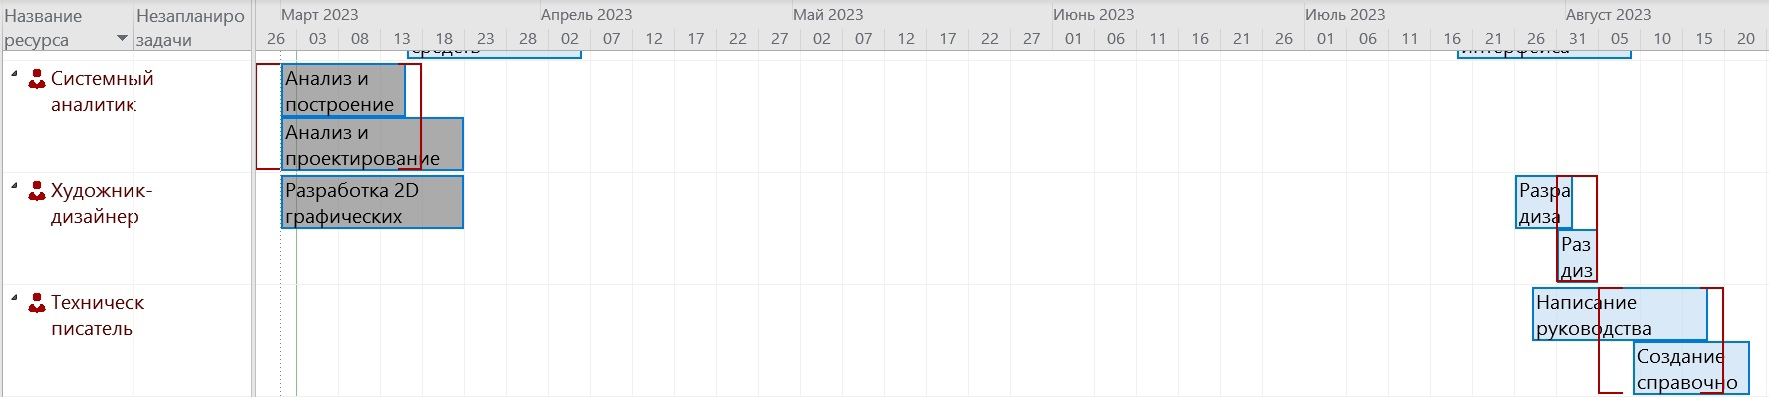
\includegraphics[scale=0.26]{inc/img/task2-overload.jpg}
	\end{center}
	\captionsetup{justification=centering}
	\caption{Возникновение перегрузок}
	\label{img:task2-overload}
\end{figure}

Появление перегрузки для ресурса <<Системный аналитик>> связано с тем, что данный ресурс задействован при выполнении задач <<Анализ и построение структуры базы объектов>> и <<Анализ и проектирование ядра>>, сроки реализаций которых накладываются.

Появление перегрузки для ресурса <<Художник-дизайнер>> связано с тем, что данный ресурс задействован при выполнении задач <<Разработка дизайна руководства>> и <<Разработка дизайна сайта>>, сроки реализаций которых накладываются.

Появление перегрузки для ресурса <<Технический писатель>> связано с тем, что данный ресурс задействован при выполнении задач <<Написание руководства пользователя>> и <<Создание справочной системы>>, сроки реализаций которых накладываются.

Назначение фиксированных затрат (1000 рублей) задачам 2, 8 и 12 приведено на рисунке \ref{img:task2-fixed-costs}.

\begin{figure}[H]
	\begin{center}
		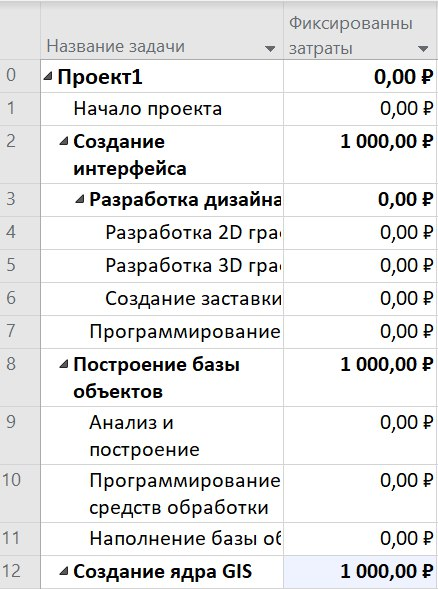
\includegraphics[scale=0.42]{inc/img/task2-fixed-costs.jpg}
	\end{center}
	\captionsetup{justification=centering}
	\caption{Назначение фиксированных затрат}
	\label{img:task2-fixed-costs}
\end{figure}

Так как для реализации задачи <<Построение базы объектов>> был арендован сервер, использующийся и днем, и ночью, по ставке два рубля в час, в ресурсный лист был добавлен трудовой ресурс <<Сервер>>, как показано на рисунке \ref{img:task2-server}.

\begin{figure}[H]
	\begin{center}
		
\includegraphics[scale=0.5]{inc/img/task2-server.jpg}
	\end{center}
	\captionsetup{justification=centering}
	\caption{Добавление ресурса <<Сервер>> в лист ресурсов}
	\label{img:task2-server}
\end{figure}

Назначение сервера задаче 8 представлено на рисунке \ref{img:task2-assignment}.

\begin{figure}[H]
	\begin{center}
		
\includegraphics[scale=0.5]{inc/img/task2-assignment.jpg}
	\end{center}
	\captionsetup{justification=centering}
	\caption{Назначение сервера задаче <<Построение базы объектов>>}
	\label{img:task2-assignment}
\end{figure}

\section*{Задание 3}

Была проведена структуризация затрат по группам ресурсов, как приведено на рисунке \ref{img:task3-costs}. Графическое представление информации о затратах по структурным группам ресурсов показана на рисунке \ref{img:task3-costs-graph}.

\begin{figure}[H]
	\begin{center}
		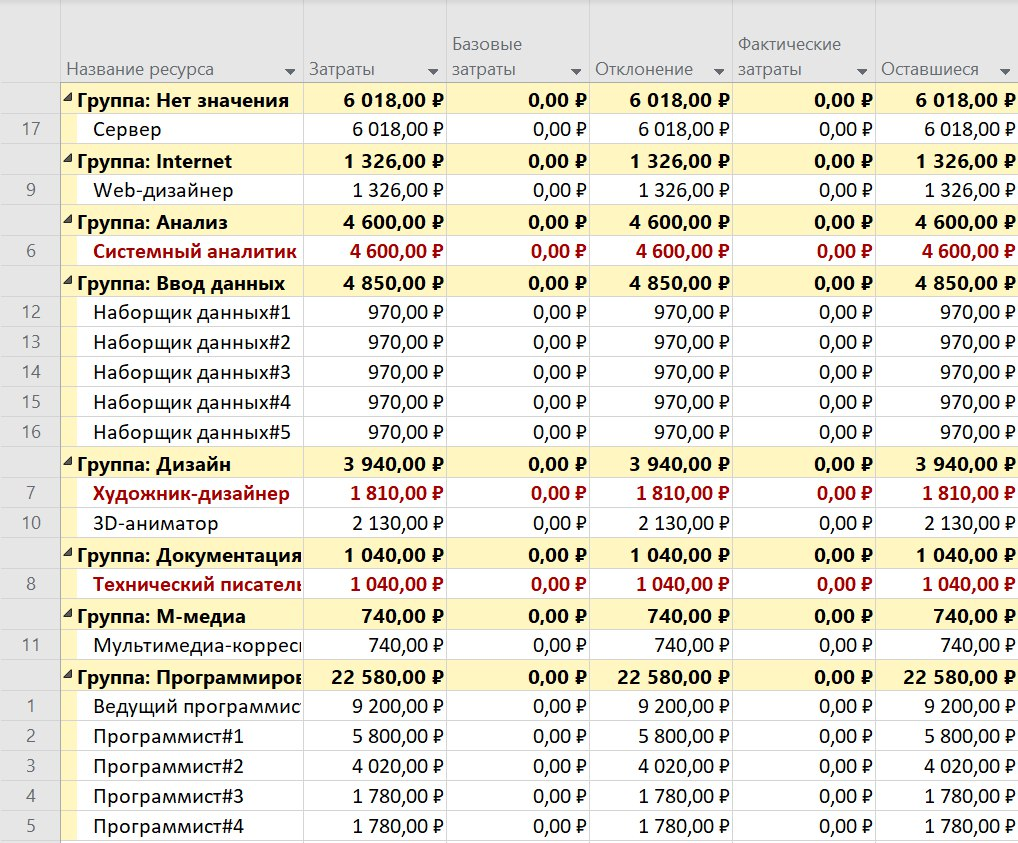
\includegraphics[scale=0.4]{inc/img/task3-costs.jpg}
	\end{center}
	\captionsetup{justification=centering}
	\caption{Структуризация затрат по группам ресурсов}
	\label{img:task3-costs}
\end{figure}

\begin{figure}[H]
	\begin{center}
		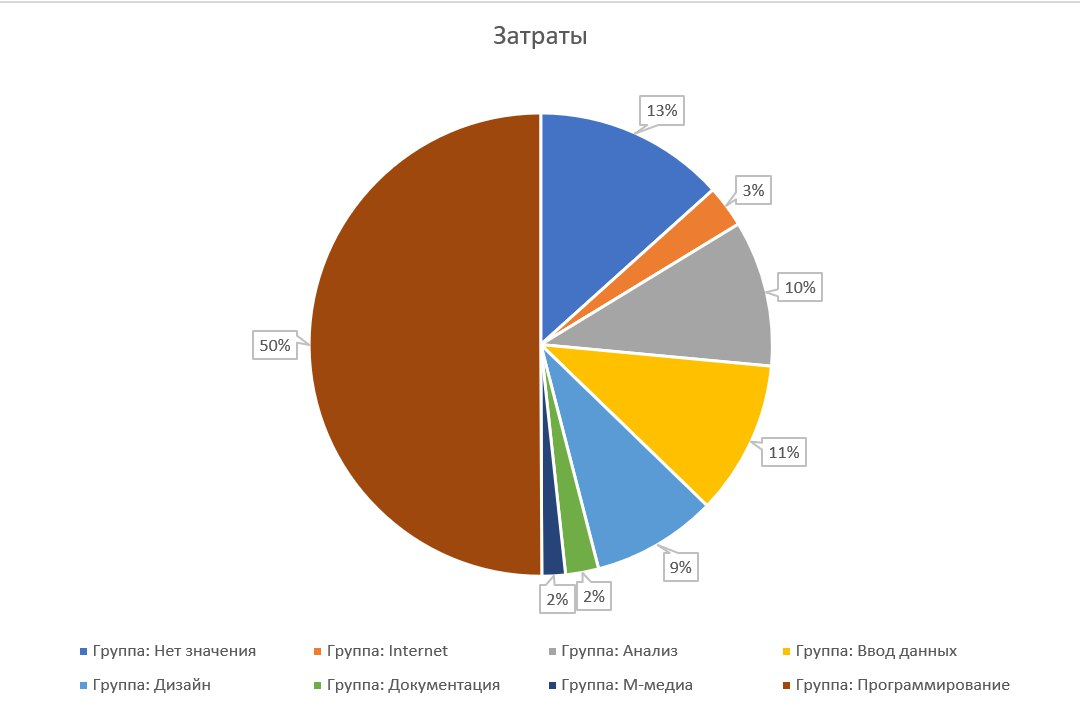
\includegraphics[scale=0.5]{inc/img/task3-costs-graph.jpg}
	\end{center}
	\captionsetup{justification=centering}
	\caption{Информации о затратах по структурным группам ресурсов}
	\label{img:task3-costs-graph}
\end{figure}

Была проведена структуризация трудозатрат по группам ресурсов, как представлено на рисунке \ref{img:task3-labor-costs}. Графическое представление информации о трудозатратах по структурным группам ресурсов приведена на рисунке \ref{img:task3-labor-costs-graph}.

\begin{figure}[H]
	\begin{center}
		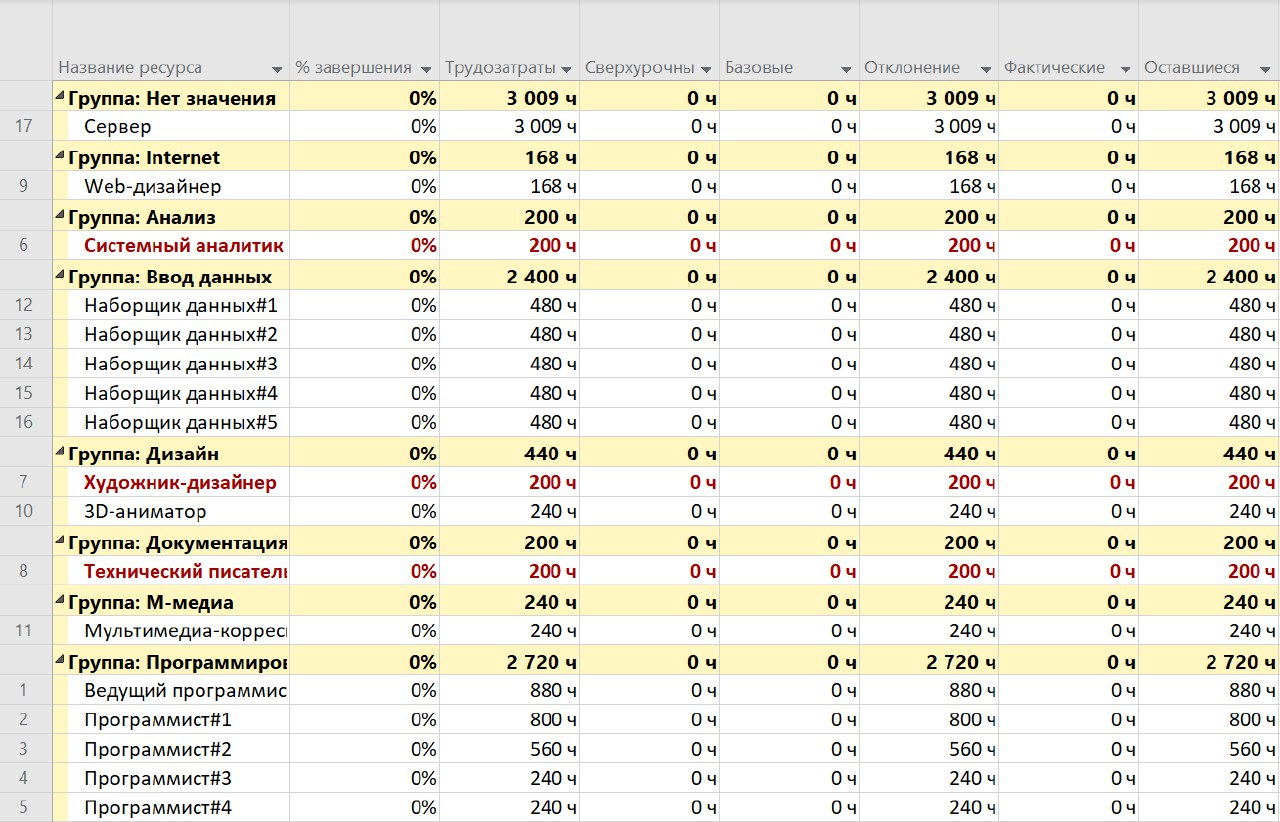
\includegraphics[scale=0.4]{inc/img/task3-labor-costs.jpg}
	\end{center}
	\captionsetup{justification=centering}
	\caption{Структуризация трудозатрат по группам ресурсов}
	\label{img:task3-labor-costs}
\end{figure}

\begin{figure}[H]
	\begin{center}
		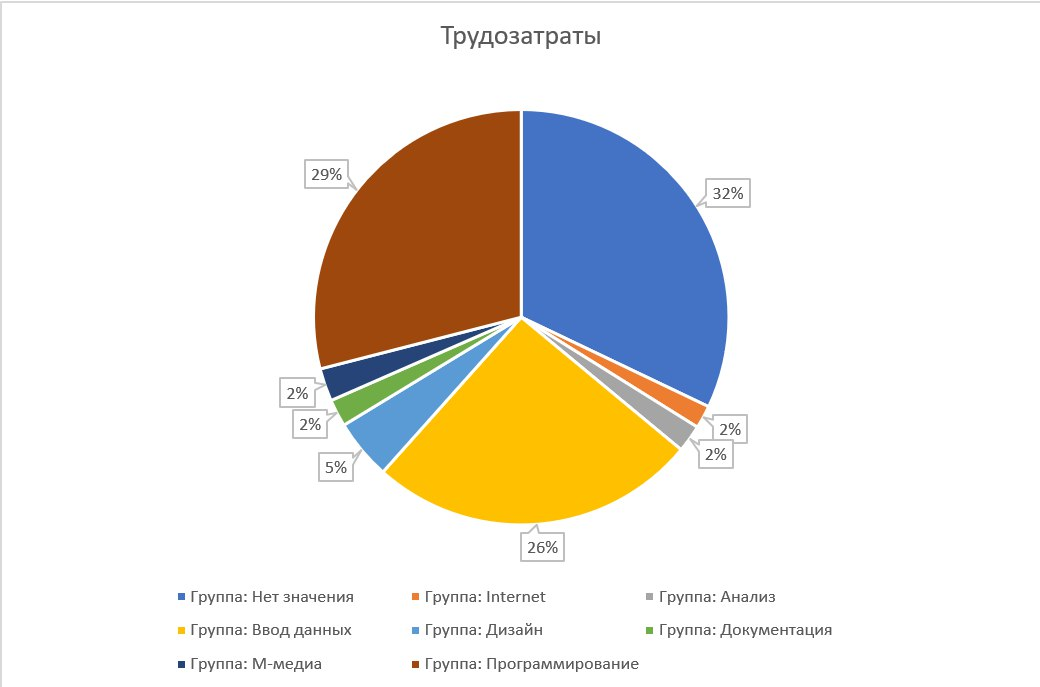
\includegraphics[scale=0.5]{inc/img/task3-labor-costs-graph.jpg}
	\end{center}
	\captionsetup{justification=centering}
	\caption{Информации о трудозатратах по структурным группам ресурсов}
	\label{img:task3-labor-costs-graph}
\end{figure}

Изучив диаграммы, демонстрирующие распределение затрат и трудозатрат проекта, можно сделать следующие выводы:
\begin{enumerate}
	\item Затраты больше на 21\% трудозатрат у ресурсов, составляющих группу <<Программирование>>. При этом затраты данных ресурсов составляют половину затрат на проект, а трудозатраты составляют 29\% трудозатрат проекта.
	\item Затраты больше на 15\% трудозатрат у ресурсов, составляющих группу <<Ввод данных>>. При этом трудозатраты данных ресурсов составляют 26\% трудозатрат проекта, а затраты составляют 11\% затрат проекта.
	\item Затраты больше на 8\% трудозатрат у ресурсов, составляющих группу <<Анализ>>.
	\item Затраты больше на 4\% трудозатрат у ресурсов, составляющих группу <<Дизайн>>.
	\item Процент затрат незначительно (1\%) отличается от процента трудозатрат у ресурсов, составляющих группу <<Internet>>.
	\item Процент затрат совпадает с процентом трудозатрат у ресурсов, составляющих группы <<М-медиа>> и <<Документация>>.
	\item Трудозатраты сервера составляет около трети (32\%) трудозатрат проекта.
\end{enumerate}

На рисунке \ref{img:task3-budget} показаны затраты и трудозатраты на проект.

\begin{figure}[H]
	\begin{center}
		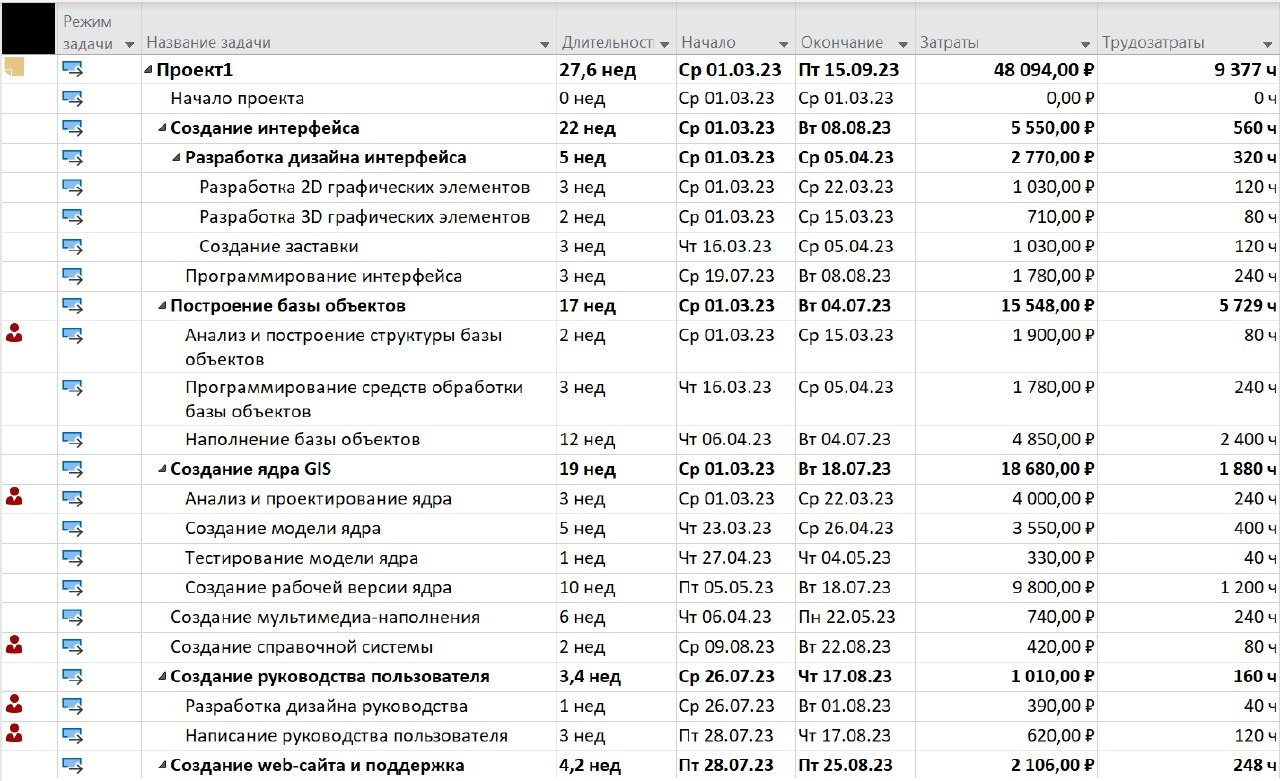
\includegraphics[scale=0.42]{inc/img/task3-budget.jpg}
	\end{center}
	\captionsetup{justification=centering}
	\caption{Затраты и трудозатраты на проект}
	\label{img:task3-budget}
\end{figure}

Из полученного результата видно, что затраты на проект составили 48~094 рублей при трудозатратах --- 9 377 часов.

\section*{Вывод}

При выполнении лабораторной работы были освоены возможности программы Microsoft Project для работы с ресурсами.

Распределение ресурсов по задачам показало, что некоторые ресурсы перегружены.

В ходе анализа затрат и трудозатрат по структурным группам ресурсов было выявлено, что не у всех групп ресурсов процент затрат и процент трудозатрат совпадают.

Из результатов планирования видно, что выделенный бюджет покрывает затраты на проект.